\section{Teilversuch 3: Qualitative Betrachtung des Spektrums von Cadmium}
	\begin{figure}[!ht]
	    \centering
	    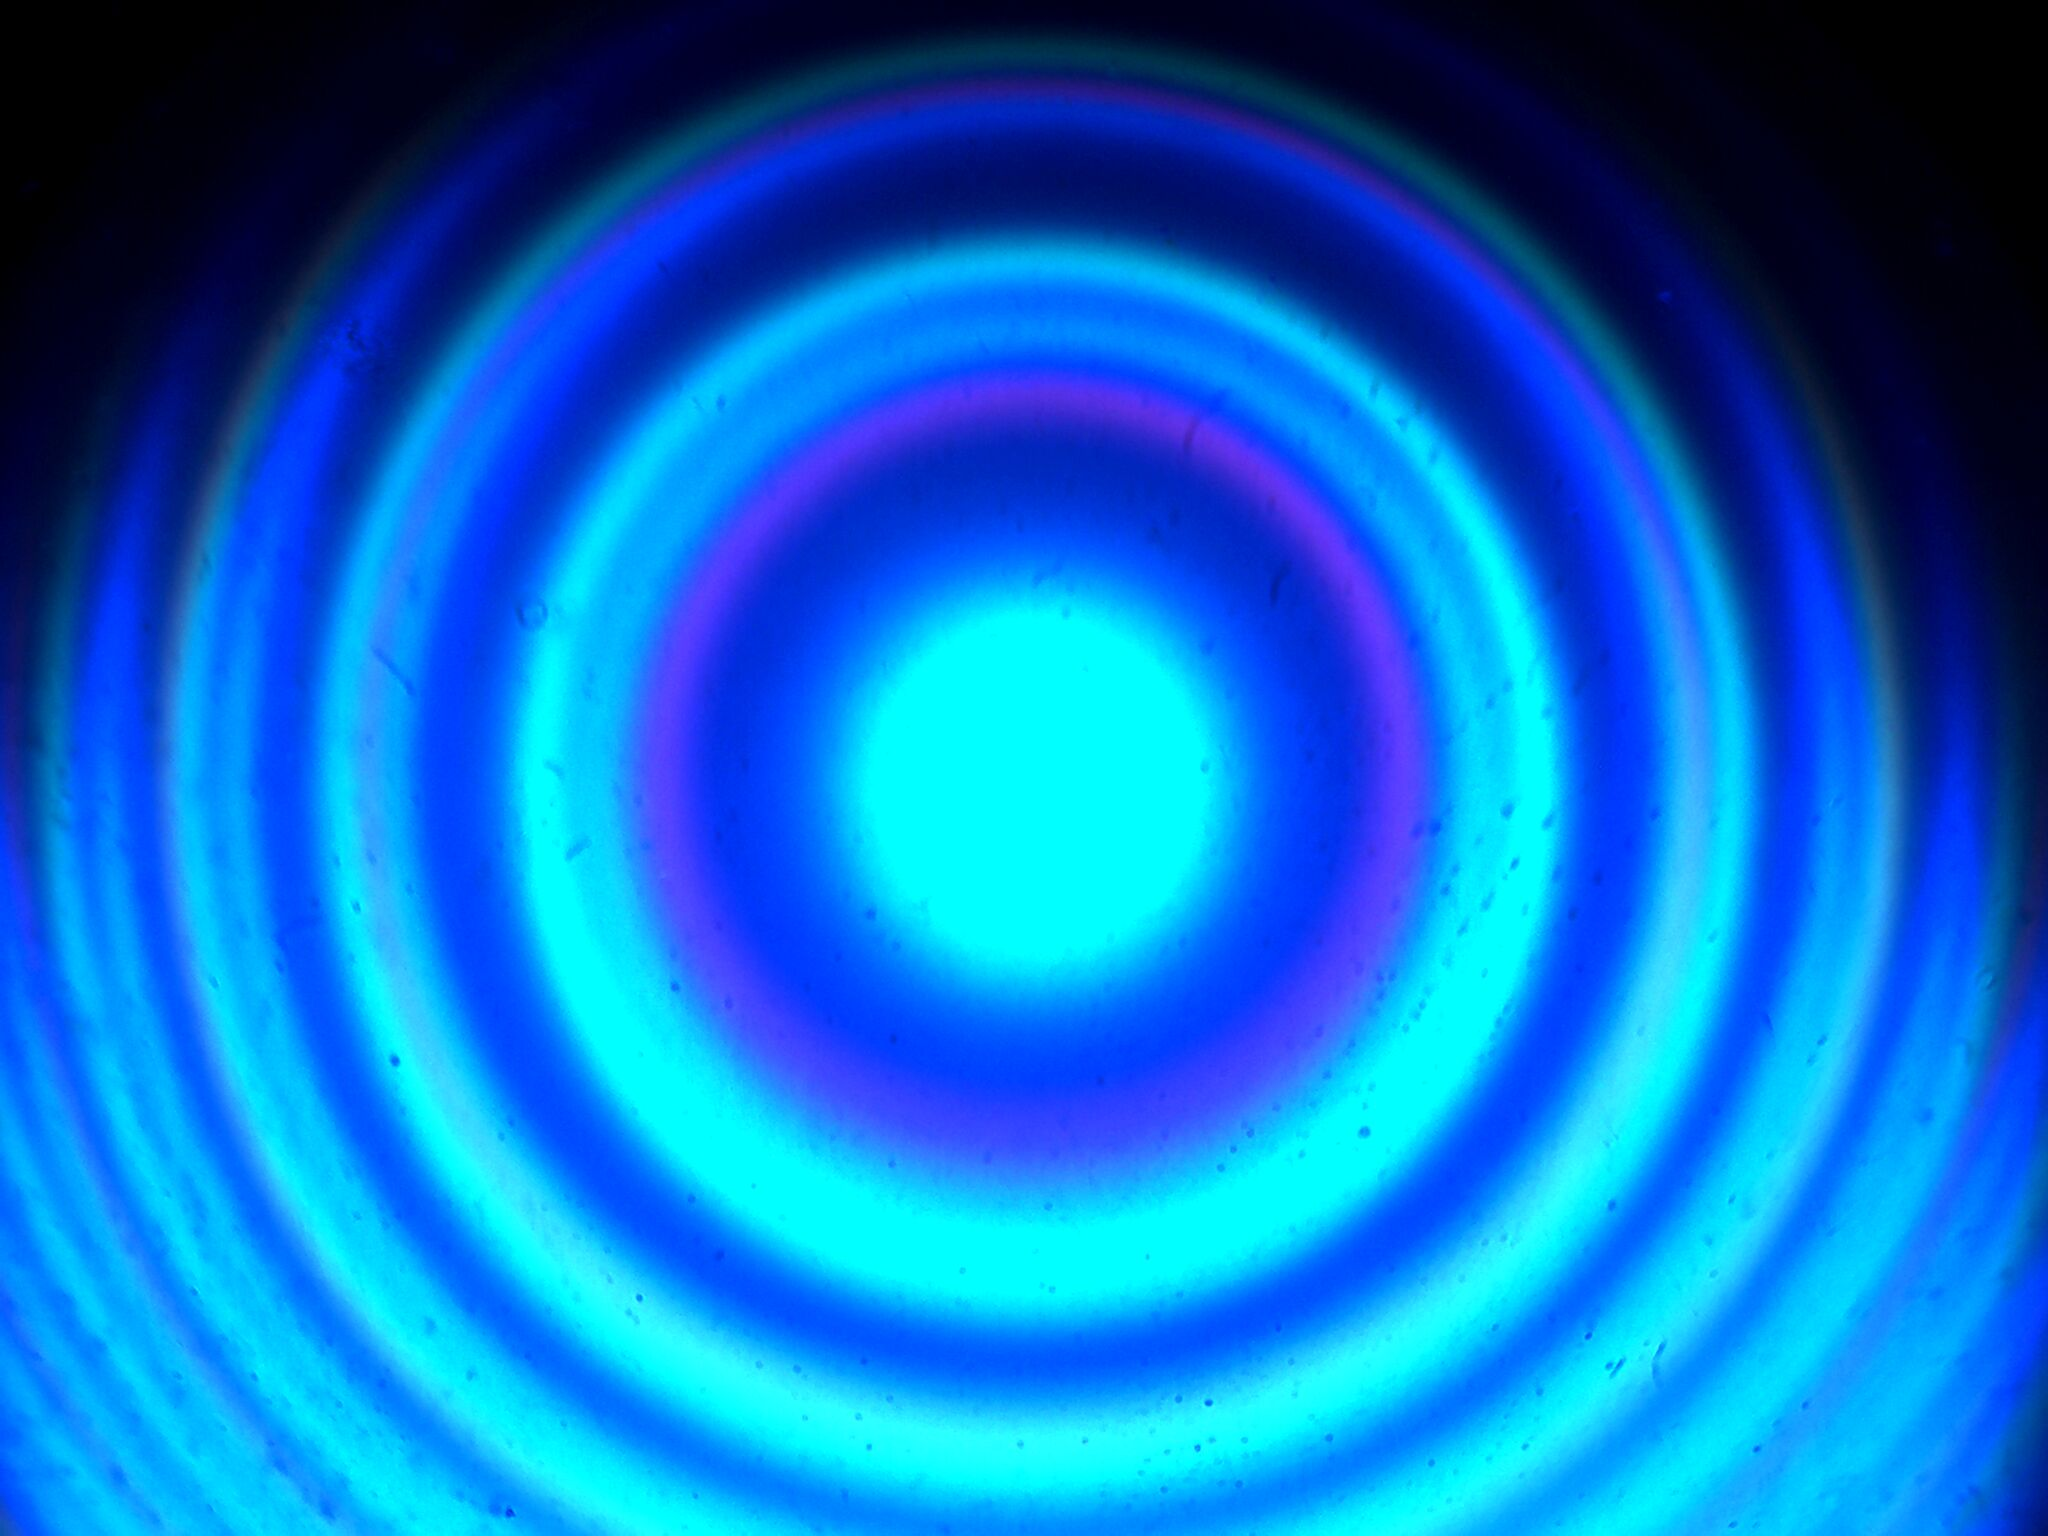
\includegraphics[width=0.45\textwidth]{images/Capture_808.bmp.jpg}
	    \hspace{1em}
	    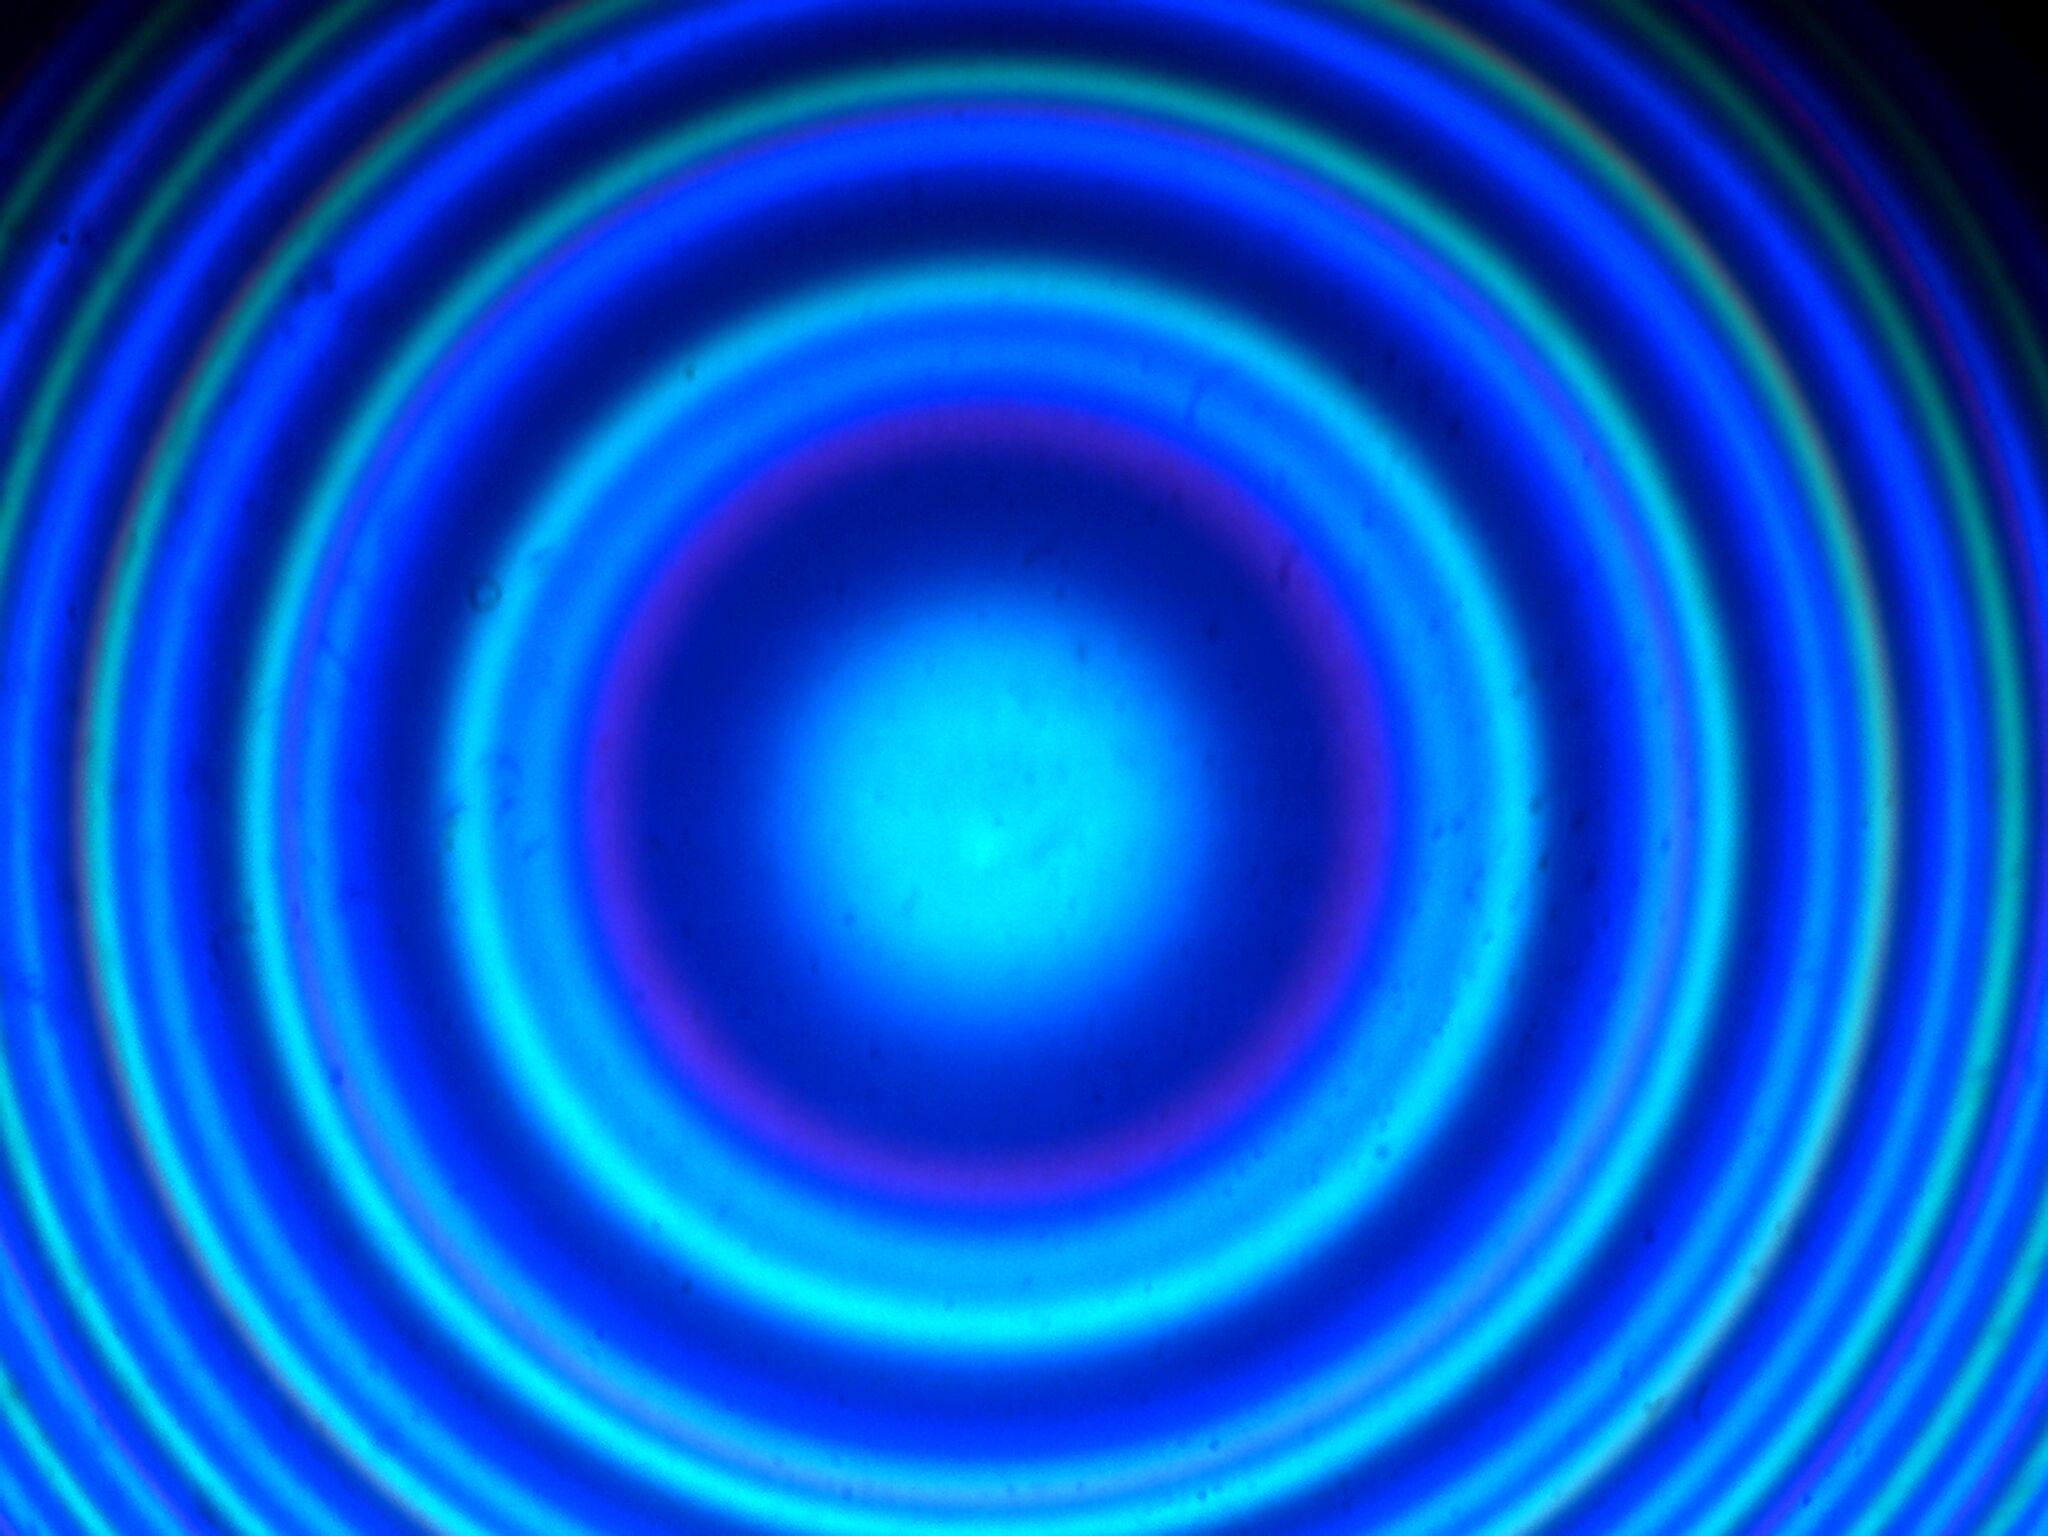
\includegraphics[width=0.45\textwidth]{images/Capture_809.bmp.jpg}
	    \caption{Interferenzringe mit Cd-Lampe. Vor Justierung (Links). Nach Justierung (Rechts)}
	    \label{fig:laser-interference}
	\end{figure}
	Es ist zu bemerken, dass ohne Kamera ist das Interferenzmuster schwer zu sehen. Laut Abbildung 1 der Anleitung gibt es nur 5 Übergängen, die im sichtbaren Bereich liegt. Wir nehmen nun an, dass die Kamera auch nur Licht im sichtbaren Bereich abbilden kann. 
	\newpage
	Die Zuordnung ist somit:
	\begin{figure}[!ht]
	    \centering
	    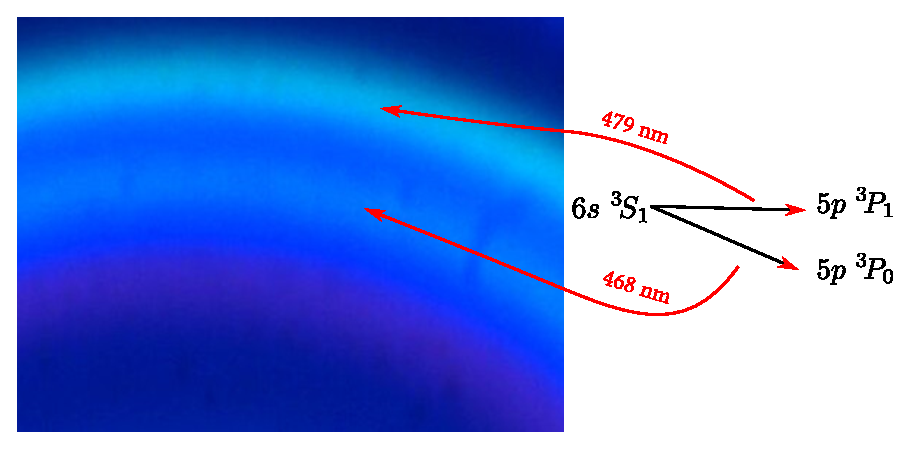
\includegraphics{images/tv3.eps}
	    \caption{Zuordnen der sichtbaren Emissionslinien}
	    \label{fig:zuordnen}
	\end{figure}

	Die andere sichtbare Linien (\SI{508.59}{\nano\meter}, \SI{515.47}{\nano\meter}, \SI{643.85}{\nano\meter}) sind wahrscheinlich zu schwach, um in diesem Bild zu sehen. Man sieht hier auch zusätzlich eine lila Emissionslinie. Sie liegt vermutlich im unsichtbaren UV Bereich ($\SI{300}{\nano\meter} < \lambda < \SI{450}{\nano\meter}$). Da es mehrere Emissionslinie in diesem Bereich liegt, lässt diese Linie nicht so gut zuordnen.


